\label{chap3}

This chapter details the parameter identification of the soft robotic actuator. First, material properties and dimensions of the soft robotic manipulator are provided. Then, determination of actuator stiffness is explained. Consequently, pressure to force input mapping is explained. Lastly, estimation of the damping parameters are detailed.


This chapter explains the approach in determining stiffness properties of the soft robotic manipulator. These properties are determined with the aid of Finite Element Analysis (FAE). Apart from stiffness properties, an input mapping is obtained. This mapping, maps the physical inputs of actuator the input used in the model.

\section{Material parameters}

\todo{op \url{https://abaqus-docs.mit.edu/2017/English/SIMACAEMATRefMap/simamat-c-hyperelastic.htm} staat meer uitgelegd}

Since the robotic manipulator is manufactured by an external company, material parameters are classified. As far as is known, the Young's Modulus $E$ is equal to $69$ MPa and Poisson ration $\nu$ is $0.45$. Furthermore, it is assumed that robotic manipulator deforms non-linearly following Neo-Hookeon behaviour. Both material parameters allows to calculate shear modulus $\mu$ and bulk modulus $\kappa$ as,

\begin{equation}
    \mu = \frac{E}{2(1+\nu)}   \hspace{50pt}  \kappa = \frac{E}{3(1-2\nu)}.
\end{equation}

\todo{For consistency with linear elasticity these moduli are reformulated as $C_{10} = \frac{\mu}{2}$  and $D_{1} = \frac{2}{\kappa}$.}


\todo{add density, maybe use cad model to determine volume, and scale to determine mass. $\rho = \frac{mass [kg]}{V [m^3]}$}{}

\section{Finite Element Analysis (FEA)}

In an effort to determine stiffness properties, finite element software
\verb+Abaqus/CAE+ is used.Various loads can be applied to the computer model of the soft actuator. By studying the deformation induced by the loads, stiffness properties can be approximated. Figure () shows the model in the finite element software. In the analysis, the bottom plate of the actuator will be constrained in all directions of motion and rotation. Furthermore, the out-of-plane motion of the actuator is not considered since the body is symmetric, and applied loads act perpendicular to this motion. A mesh refinement analysis has been done to determine an accurate mesh size, see Appendix \ref{app:chap3}. For determining the stiffness properties gravitational effects are omitted. An elongation and curvature analysis of the robot manipulator is considered. These help to obtain elongation and rotation stiffness, respectively. The results of the FEA are further processed in Matlab. The process of acquiring nodal information from \verb+Abaqus/CAE+ is further elucidated in Appendix \ref{app:chap3}. The post-processing of this data in Matlab is explained in Section \ref{sec3:KinematicModelFit}  \todo{write appendix on data post processing}



\subsection{Elongation analysis}


The elongation analysis aims to measure pure elongation of the soft actuator. This allows for determining elongation stiffness, as rotating effects of the top of the robot are small. ``Pure'' elongation is induced by pressurizing both bellows equally. By doing this for a set of different pressures, a relation between elongation and pressure can be found. Figure (\ref{fig3:elongationvspressure}) shows the relation between elongation function of pressure. Additionally, the curvature of the manipulator is shown for various pressures. It can be seen that pressurizing the bellows equally results in a near pure elongation. This allows to determine the elongation stiffness as effects of rotation are deemed negligible. The elongation rate decreases as pressure increases, this is the result of a non-linear material parameters. Before the non-linear stiffness can be determined, the pressure to force mapping should be found. This is discussed in Section \ref{sec3:InputMapping}.

\begin{figure}[H]
    \centering
\begin{minipage}{0.5\textwidth}
        \centering
        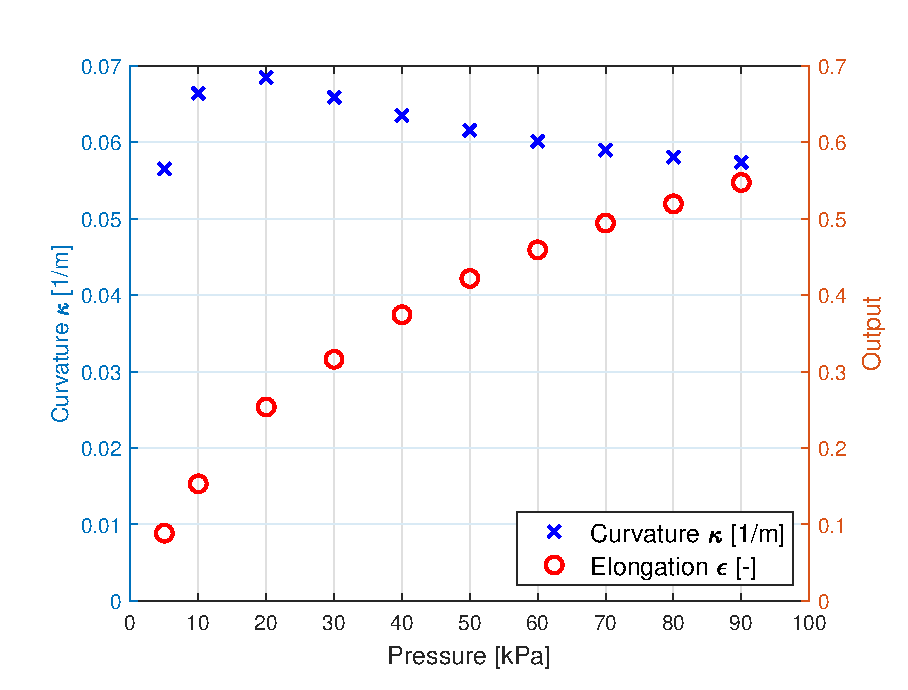
\includegraphics[width=\textwidth]{Figures/Chapter3/elongationvspressure.eps} 
        \caption{Elongation analysis, elongation and curvature as function of pressure.}
        \label{fig3:elongationvspressure}
    \end{minipage}\hfill
    \begin{minipage}{0.5\textwidth}
        \centering
        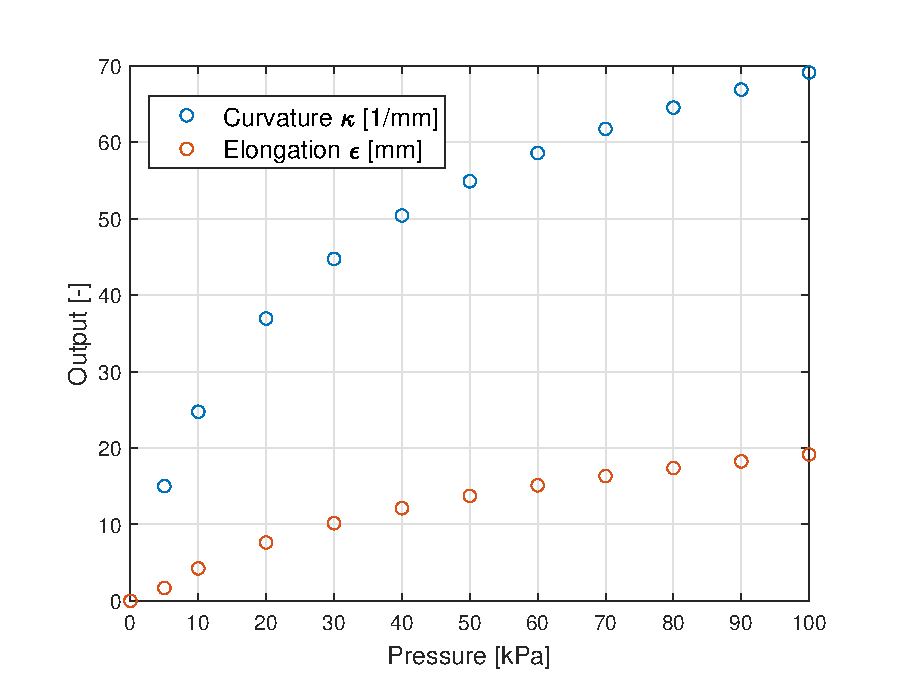
\includegraphics[width=\textwidth]{Figures/Chapter3/rotationvspressure.eps} 
        \caption{Curvature analysis, elongation and curvature as function of pressure.}
        \label{fig3:rotationvspressure}
    \end{minipage}
\end{figure}

\todo{mention the coupling?}
\subsection{Curvature analysis}

The curvature analysis allows to determine rotation stiffness of the robot manipulator. For this analysis only a single bellow is pressurized, while the other bellow pressure is kept zero. The pressurized bellow will result in a force. This force induces a moment around the center of the actuator, causing the actuator to curve. This results in a curvature as well as an elongation of the backbone curve. The result of this analysis is shown in Figure \ref{fig3:elongationvspressure}. It can be seen that the curvature and elongation rates decrease as pressure increases. From this experiment the rotation stiffness can be determined when the input mapping is known.  


\section{Kinematic Model Fit}
\label{sec3:KinematicModelFit}

The acquired data from the FEA is post-processed in Matlab to estimate the elongation and curvature of the analysis. This is done with the aid of the developed kinematic model. The kinematic model will be fitted through the nodal output of the FEA. The user can define the amount of shape functions used to approximate the shape of simulations. Increasing the amount of shape-functions will result in more flexibility. Therefore it can describe the actual deformation pattern better. However, fairly accurate approximations can be obtained when using a single-shape function. This means that each free strain, e.g. elongation and curvature, is described with a shape function polynomial of degree 1. Implying that the modal coordinates can be expressed as in Equation (\ref{eq3:q}). Expressing the curvature of the manipulator
 $\kappa \in \mathbb{R}$ $[\frac{1}{m}]$ . and elongation $\epsilon \in \mathbb{R}$ $[m]$.  This means that the simulation results are approximated using the constant curvature approach.

\begin{equation}
    q =  \begin{bmatrix} q_1 \\ q_2 \end{bmatrix}     = \begin{bmatrix} \kappa \\ \epsilon \end{bmatrix} 
    \label{eq3:q}
\end{equation}




\begin{figure}[H] 
  \begin{minipage}[b]{0.5\linewidth}
    \centering
    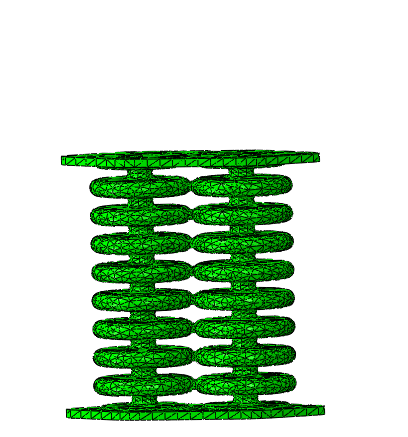
\includegraphics[width=\linewidth]{Figures/Chapter2/undeformed.png} 
    \caption{Undeformed FEA.} 
    \vspace{4ex}
    \label{fig3:FEMun} 
  \end{minipage}%%
  \begin{minipage}[b]{0.5\linewidth}
    \centering
    \includegraphics[width=\linewidth]{Figures/Chapter2/deformed60kpa.png} 
    \caption{Deformed FEA.} 
    \vspace{4ex}
    \label{fig3:FEMdef} 
  \end{minipage} 
  \begin{minipage}[b]{0.5\linewidth}
    \centering
    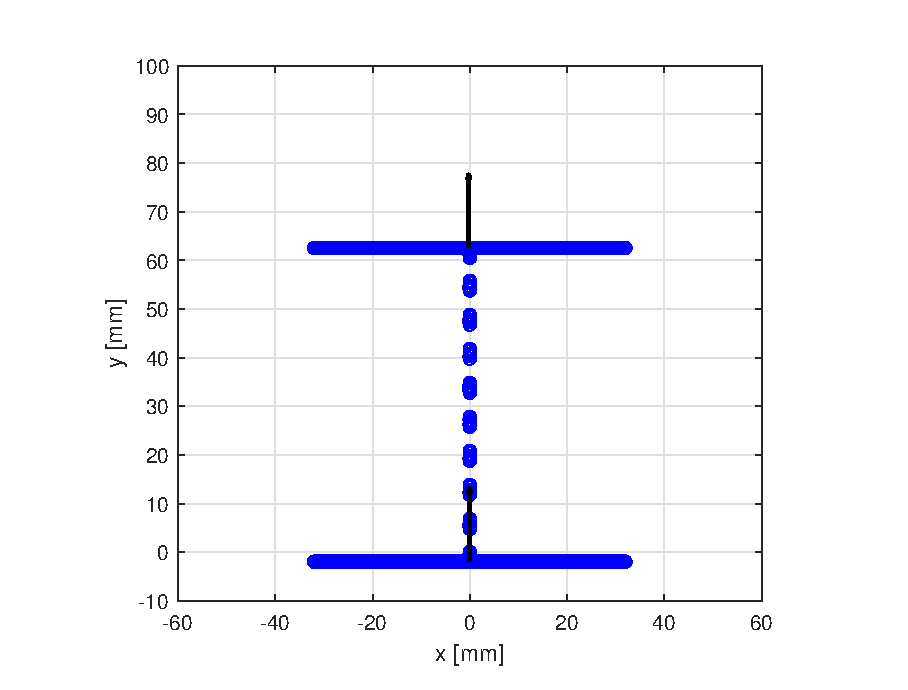
\includegraphics[width=\linewidth]{Figures/Chapter2/undeformednodal.eps} 
    \caption{Nodal image undeformed} 
    \vspace{4ex}
    \label{fig3:MATun} 
  \end{minipage}%% 
  \begin{minipage}[b]{0.5\linewidth}
    \centering
    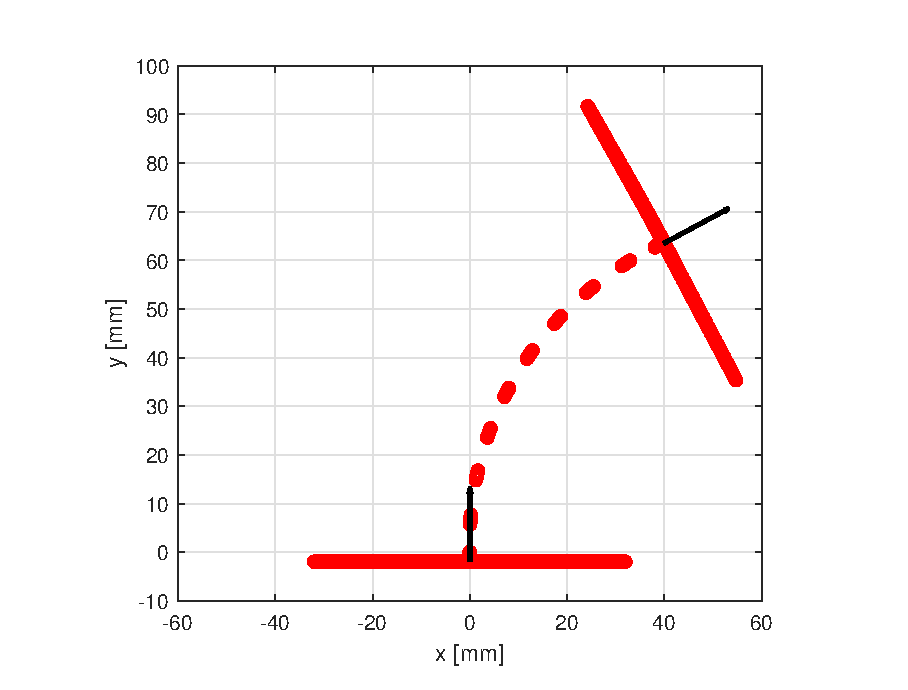
\includegraphics[width=\linewidth]{Figures/Chapter2/deformednodal.eps} 
    \caption{Nodal image deformed } 
    \vspace{4ex}
    \label{fig3:MATdef} 
  \end{minipage} 
\end{figure}
\todo{in this figure add crosses at the center cluster of nodes representing the backbone curve}

Figures (\ref{fig3:FEMun}) and (\ref{fig3:FEMdef}) show the undeformed and deformed robotic manipulator in the finite element software, respectively. Their post-processed nodal image is shown in  Figures (\ref{fig3:FEMun}) and (\ref{fig3:FEMdef}), respectively. These images represent a curvature analysis where the left bellow is pressurized to 60 kPa. The nodal image shows clusters of nodes. The top and bottom plates, and backbone curve can clearly be distinguished. For the small clusters of nodes representing the backbone curve, the mass middle point has been determined. Denoted as 
vector  $\Bar{x}_{mid} \in \mathbb{R}^{2\times n}$ containing the coordinates of each mass middle point. The approximate length of the backbone curve can be determined by using the function \verb+arc_length.m+ \cite{arclength}. This functions uses vector $\Bar{x}_{mid}$  to approximate the arc length of this collection of coordinates. This estimated arc length is represented as  $\Bar{x}_{length} \in \mathbb{R}^+ $ is Matlab function \verb+affine_fit.m+ \cite{affinefit} is used to determine the orientation of the plane, hence the displayed normal vectors. Additionally, this function determines the mass middle point of the cluster of nodes representing the top plate. This point will be denoted as $\Bar{x}_{end} \in \mathbb{R}^{2\times 1}$representing the coordinate of the end-effector.

An inverse kinematic configuration can fitted through the nodal displacement data. This is done via optimization with \verb+fmincon.m+  To this end, the actuator is scaled to have length 1. This can be done by dividing all coordinates by the actuator length. The minimization problem that follows is,


\begin{equation}
\begin{aligned}
\min_{q} \hspace{5pt}  q^\top Q q  + \sum_{i=1}^{N}[\Phi_1(\Bar{x}_{mid} - f(q))^2] +   \Phi_2(\Bar{x}_{end}  - f(q)_{end})^2 +  \Phi_3(\Bar{x}_{length} - & f(q)_{length})^2  \\ 
\text{s.t.} \hspace{5pt} \epsilon - 1 > 0
\end{aligned}
\end{equation}


where $Q$ is $\text{diag}([0.01,1])$ is a diagonal weighing matrix used to penalize the value of the modal coordinates. This matrix $Q$ is tuned to penalize high values of $q$.  Additional weighing factors $\Phi_i \in \mathbb{R}^+$ and $i \in \{1,2,3\}$ are applied to penalize individual terms and equal to $1e5$,$1e5$ and $5e4$, respectively. The imposed constrained affects the elongation of the manipulator. Physically this constraint implies that the actuator can shorten in length, but the length can not become negative.

Figure (\ref{fig3:nodalfitelong}) and (\ref{fig3:nodalfitcurv}) show the result of fitting the inverse kinematic model through a set of nodal data. Figure (\ref{fig3:nodalfitelong}) shows a elongation analysis were both bellows are pressurized to 60 kPa. The modal coordinates belonging to this fit are  $q = [0.06, 0.45]^\top$. The obtained modal coordinate expressing curvature again stresses the small curvature introduced with this analysis. Figure (\ref{fig3:nodalfitcurv}) shows a curvature analysis were the left bellow is pressurized to 60 kPa. The modal coordinates belonging to this fit are $q = [14,0.24]^\top$.


\begin{figure}[H]
    \centering
\begin{minipage}{0.5\textwidth}
        \centering
        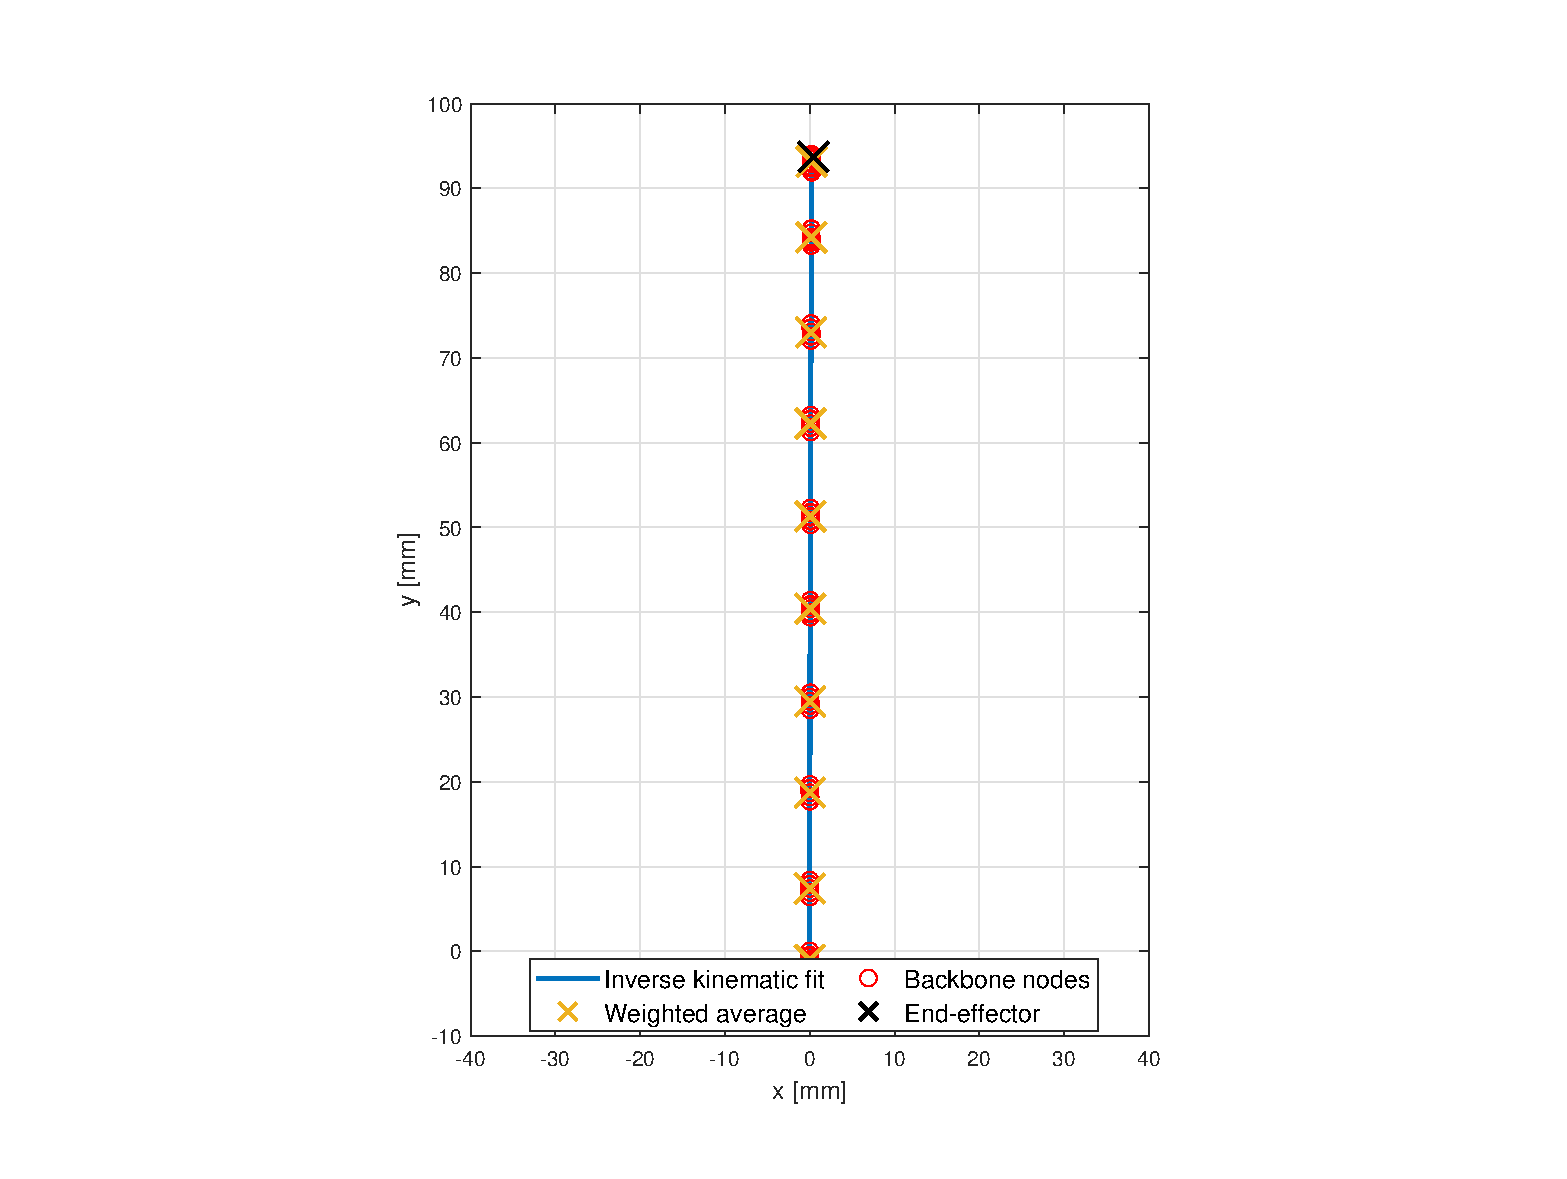
\includegraphics[width=\textwidth]{Figures/Chapter3/nodalfitelong.eps}
        \caption{Inverse kinematic fit for an elongation analysis. Both bellows pressurized to 60kPa.}
        \label{fig3:nodalfitelong}
    \end{minipage}\hfill
    \begin{minipage}{0.5\textwidth}
        \centering
        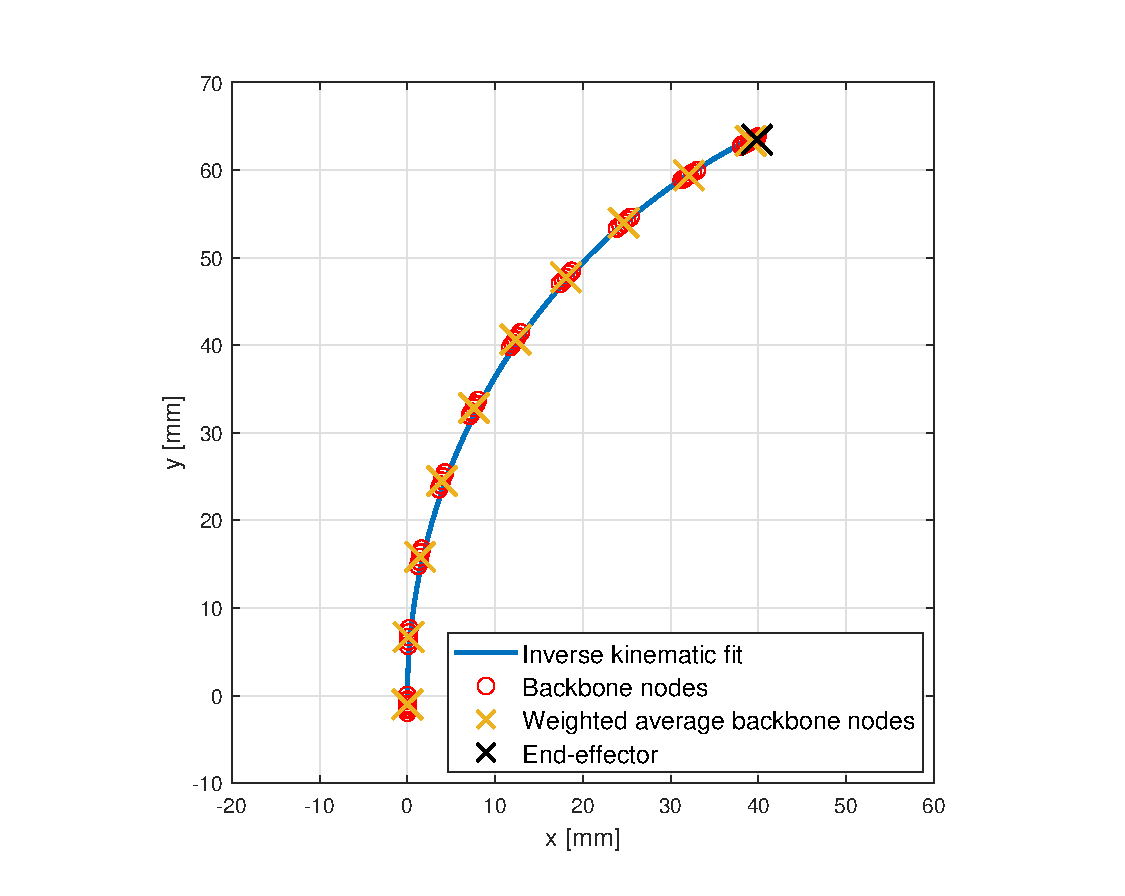
\includegraphics[width=\textwidth]{Figures/Chapter3/nodalfit.eps} 
        \caption{Inverse kinematic fit for a curvature analysis. Left bellow pressurized to 60kPa.}
        \label{fig3:nodalfitcurv}
    \end{minipage}
\end{figure}







\section{Input mapping}
\label{sec3:InputMapping}

Stiffness is the ratio between applied force and elongation. To determine  stiffness for elongation and curvature, applied forces and direction of deformation is necessary. For the physical set-up, individual bellow pressure $p_i \in \mathbb{R}^{\geq 0}$ with $i$ $\mathbb{N} \in \{1,2\}$ can be regulated. However, the control input in the dynamic model is force $F \in \mathbb{R}$ and moment $M \in \mathbb{R}$. Therefore, $H \in \mathbb{R}^{2 \times 2}$ is necessary to perform mapping $p \mapsto F$ and $p \mapsto M$ as,

\begin{equation}
     \begin{bmatrix} F \\ M \end{bmatrix}     = \underbrace{\begin{bmatrix}  a_1 & a_2 \\ a_3 & a_4 \end{bmatrix}}_{H}         \begin{bmatrix}  p_1 \\ p_2 \end{bmatrix}, \label{eq3:H}
\end{equation}

where entries of $H$ are to be determined. Our aim is to decouple rotation and elongation. Therefore, it is important to understand that $F$ causes elongation of the soft robotic actuator. Whereas, $M$ results in a curvature of the actuator. Therefore, the entries of $a_1$ and $a_2$ represent an effective surface area on which the pressure acts. Constant $a_3$ and $a_4$ represent a combination of effective surface area and lever on which the force acts. Due to symmetry properties it must hold that $a_1 = a_2$ and $a_3 = -a_4$.

First, the relation between pressure and force tried to be obtained. This will be done by using the finite element software again. The idea is to map pressure to force by using elongation. Pressurizing both bellows equally, resulted in almost ``pure" elongation. Effectively, the same result can be achieved by applying an equally distributed force on the top plate of the actuator. To this end, simulations for a set of forces applied to the top of actuator are simulated. The results for this simulation are presented in Figure (\ref{fig3:forcemap}). The horizontal axis show the modal coordinates, determined using the inverse kinematic fit as discussed previously. The contribution to the curvature is for both pressure and force simulation is again small. The scaling of the of the vertical axis already reveals that a linear relation can be found.


\begin{figure}[H]
    \centering
\begin{minipage}{0.5\textwidth}
        \centering
        \includegraphics[width=\textwidth]{Figures/Chapter3/forcepressuremodal.eps}
        \caption{Modal coordinates $\kappa$ and $\epsilon$ for elongation analysis and force analysis.}
        \label{fig3:forcemap}
    \end{minipage}\hfill
    \begin{minipage}{0.5\textwidth}
        \centering
        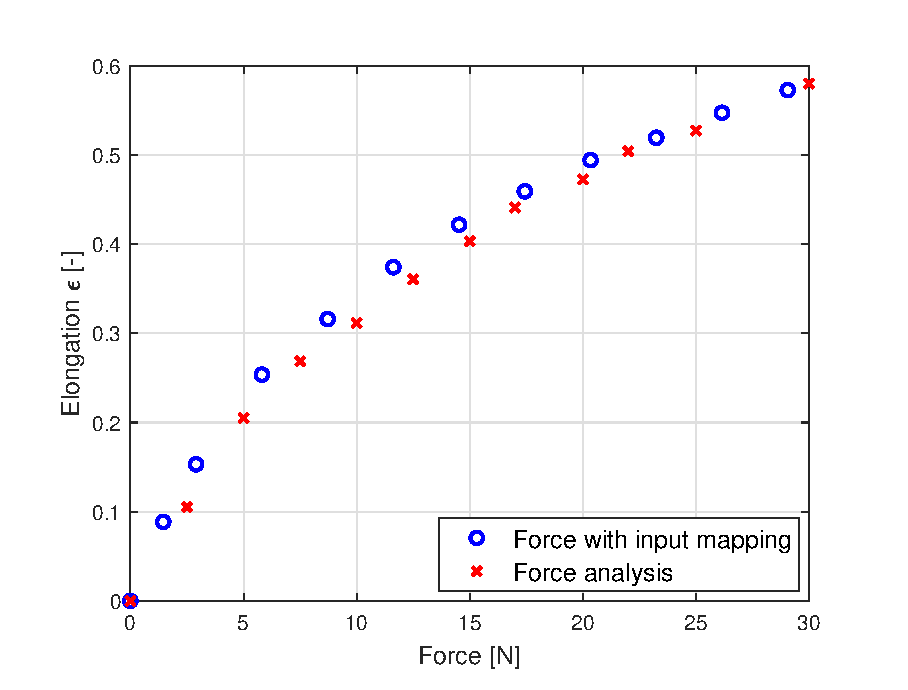
\includegraphics[width=\textwidth]{Figures/Chapter3/pressureforceelongation.eps} 
        \caption{Elongation expressed for force analysis and force with input mapping.}
        \label{fig3:forcetopressure}
    \end{minipage}
\end{figure}

The linear mapping coefficient, can be found by solving least squares problem as,



\begin{equation}
\min_{a_1} \sum_{i=1}^{N} (F_i - 2 a_1 p_i)^2
\label{eq3:forcefitting}
\end{equation}

were $i$ indicated each sample point. The effective pressure area is found to be equal to 0.1462. Since $a_1 = a_2$ the mapping of pressure in kilo Pascals and force in Newton is obtained. Figure (\ref{fig3:forcetopressure}) shows the results of the input mapping for the elongation. It can be seen that the pressure maps fairly accurate to the force.

Now the effective pressure area has been determined, the mapping to the moment can be calculated. It is assumed that the force acts on the top plate at a given radius form the backbone curve. The measured lever on which the force acts is equal to 12.56 mm. This allows to calculate $a_3$ and $a_4$by multiplying $a_1$ with this distance. The mapping matrix $H$ then follows as,

\begin{equation}
    H =  \begin{bmatrix} 0.14526 & 0.14526 \\1.8245e-3 & -1.8245e-3\end{bmatrix}  
\end{equation}




\section{Stiffness results}

The force mapping and the inverse kinematic fit to the FEA can be used to determine the elongation and curvature stiffness. A non-linear trend in elongation and curvature as function of pressure was already observed. Therefore, it is assumed that the stiffness can be captured by the hyper-elastic stiffness model as formulated in \cite{Caasenbrood2020StiffnessModel}. This non-linear stiffness model poses that stiffness $k(q_i) \in \mathbb{R}^{\geq 0}$ and meets condition $\underbar{$k$} < k(q_i) < \Bar{k}$. The model used to describe elongation is described by,

\begin{equation}
    K_\epsilon(\alpha,q_\epsilon) =  \alpha_1 + \alpha_2 [\tanh({\alpha_3 \epsilon})^2 -1]
\end{equation}


where $\alpha_i$ and  for $i \in \{1,2,3\} $ are positive stiffness parameters to be found. It is assumed that negative pressures, e.g. creating a vacuum, result in equal elongation yet in opposite direction. Hence, self contact of the bellows is neglected. This assumption is deemed valid as this situation will not occur with the current set-up. These parameters can be found by solving the non linear constraint optimisation described by,


\begin{equation}
\begin{aligned}
\min_{\alpha_1,\alpha_2,\alpha_3} \hspace{5pt} \sum_{i=1}^{N}(F_i -  (\alpha_1 + \alpha_2 [\tanh({\alpha_3 \epsilon_i})^2 -1])\epsilon_i)^2    \\ 
\text{s.t.} \hspace{5pt} \alpha_1 > \alpha_2 > 0 \\
\alpha_3 > 0 \\ 
\label{eq3:Keopt}
\end{aligned}
\end{equation}

which objective is to minimize the the sum of the errors between the mapped force, and force resulting from the stiffness model. As for the elongation stiffness, the curvature stiffness can be characterized by,

\begin{equation}
    K_\kappa(\beta,q_\kappa) =  \beta_1 + \beta_2 [\tanh({\beta_3 \kappa})^2 -1]
\end{equation}


where $\beta_i$ for $i \in \{1,2,3\} $ are positive stiffness parameters to be found. These parameters can be found by solving,

\begin{equation}
\begin{aligned}
\min_{\beta_1,\beta_2,\beta_3} \hspace{5pt} \sum_{i=1}^{N}(M_i -  (\beta_1 + \beta_2 [\tanh({\beta_3 {\kappa_i}})^2 -1]){\kappa_i})^2    \\ 
\text{s.t.} \hspace{5pt} \beta_1 > \beta_2 > 0 \\
\beta_3 > 0 \\ 
\label{eq3:Kkopt}
\end{aligned}
\end{equation}



where the objective is to minimize the sum of errors between the mapped moment Solving the optimization problems described in (\ref{eq3:Keopt}) and (\ref{eq3:Kkopt}) result in the stiffness parameters as presented in Table (\ref{tab3:stiffnessparameters})

\begin{table}[H]
    \centering
        \caption{Parameters for hyper-stiffness model.}
\begin{tabular}{|c|c|c|c|} \hline
            &  $i = $ 1      &    $i = $    2   &  $i = $ 3  \\ \hline
   $\alpha_i \hspace{2pt}[N]$    &    1.3936e+3    & 1.3776e+3    & 2.7865e-1 \\ \hline
   $\beta_i \hspace{2pt}  [Nm^2] $     &  3.0322 & 3.0309    &  3.3755e-3\\ \hline
\end{tabular}
    \label{tab3:stiffnessparameters}
\end{table}

Figure (\ref{fig3:elongvsforce}) shows the result of solving the regression problem of (\ref{eq3:Keopt})


\begin{figure}[H]
    \centering
\begin{minipage}{0.5\textwidth}
        \centering
        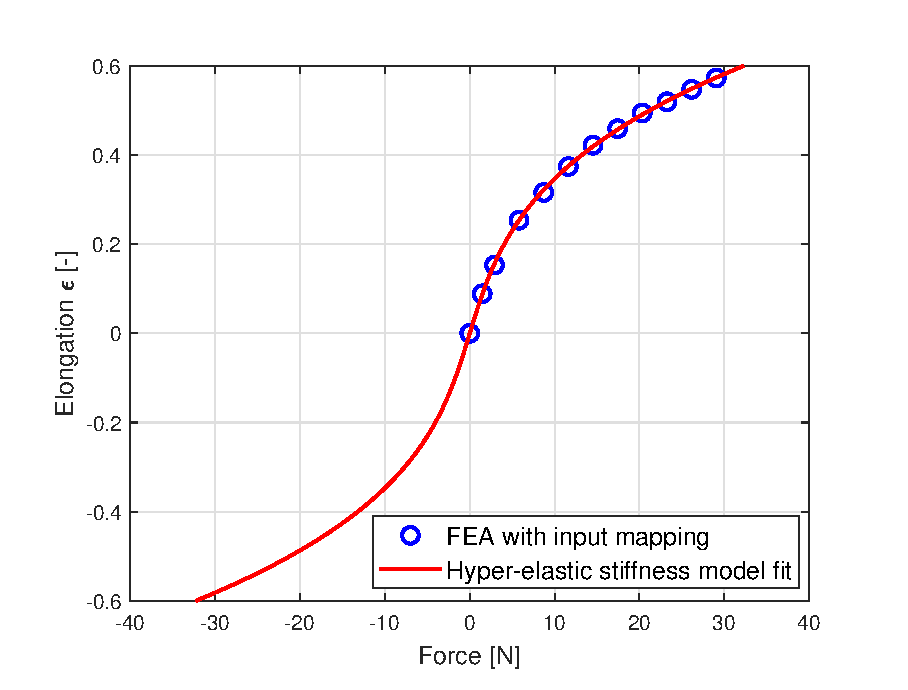
\includegraphics[width=\textwidth]{Figures/Chapter3/mappedforcevselongation.eps}
        \caption{Fitted stiffness model for elongation.}
        \label{fig3:elongvsforce}
    \end{minipage}\hfill
    \begin{minipage}{0.5\textwidth}
        \centering
        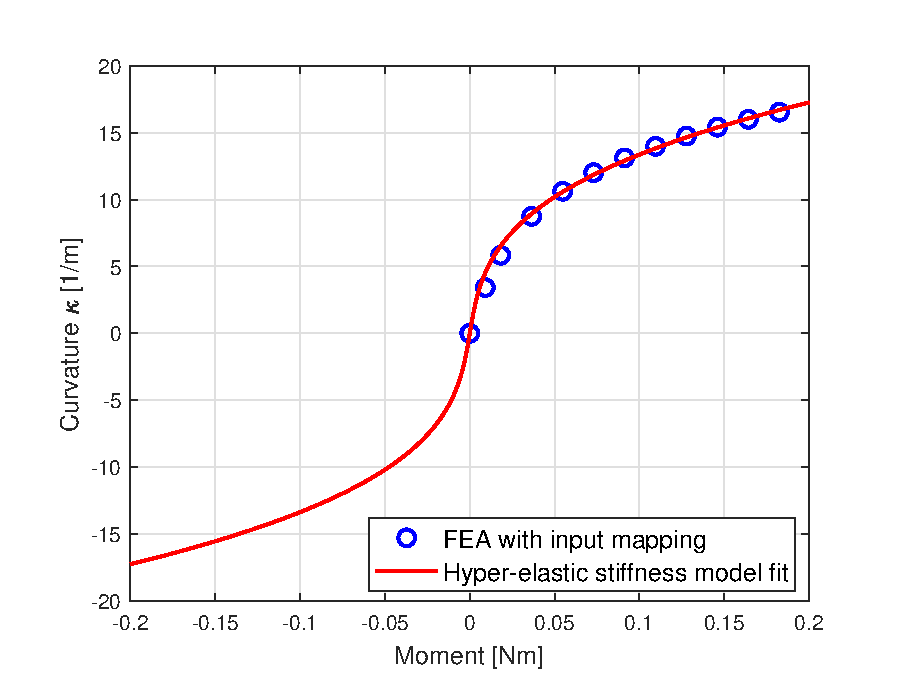
\includegraphics[width=\textwidth]{Figures/Chapter3/mappedmomentvscurvature.eps} 
        \caption{Fitted stiffness model for curvature.}
        \label{fig3:curvsmoment}
    \end{minipage}
\end{figure}

\todo{coupling is neglected}